\documentclass[12pt,t]{beamer}
\usepackage{graphicx}
\usepackage[vlined]{algorithm2e}
\usepackage{times}
\usepackage{calc}
\usepackage{url}
\usepackage{soul}
\usepackage{graphicx}
\usepackage{multirow, hhline}
\usepackage{array, booktabs}
\usepackage{amsmath}
\usepackage{amssymb}
\usepackage{relsize}
\usepackage{multirow}
\usepackage{booktabs}
\usepackage{pagecolor}
\usepackage{lipsum}
\usepackage{capt-of}
\usepackage{booktabs}

\usepackage{graphicx}
\usepackage{multicol}
\usepackage[T1]{fontenc}
\usepackage{ae}
\graphicspath{{fig/}}
\setbeameroption{hide notes}
\setbeamertemplate{note page}[plain]

\usetheme{default}
\beamertemplatenavigationsymbolsempty
\hypersetup{pdfpagemode=UseNone}

\usefonttheme{professionalfonts}
\usefonttheme{serif}
\usepackage{fontspec}
\setmainfont{Karla}
\setbeamerfont{note page}{family*=pplx,size=\footnotesize} % Palatino for notes

\definecolor{foreground}{RGB}{70,70,70}
\definecolor{background}{RGB}{249, 249, 249} %24,24,24
%\definecolor{title}{RGB}{107,174,214} %107,174,214
\definecolor{title}{RGB}{70,70,70}
\definecolor{gray}{RGB}{0,0,0}
\definecolor{subtitle}{RGB}{70,70,70}
\definecolor{hilight}{RGB}{102,255,204}
\definecolor{vhilight}{RGB}{255,111,207}

\setbeamercolor{titlelike}{fg=title}
\setbeamercolor{subtitle}{fg=subtitle}
\setbeamercolor{institute}{fg=gray}
\setbeamercolor{normal text}{fg=foreground,bg=background}


\setbeamercolor{item}{fg=foreground} % color of bullets
\setbeamercolor{subitem}{fg=gray}
\setbeamercolor{itemize/enumerate subbody}{fg=gray}
\setbeamertemplate{itemize subitem}{{\textendash}}
\setbeamerfont{itemize/enumerate subbody}{size=\footnotesize}
\setbeamerfont{itemize/enumerate subitem}{size=\footnotesize}

\setbeamercolor{block title}{fg=white,bg=gray!70}
\setbeamercolor{block body}{fg=black,bg=gray!10}
\setbeamercolor{block title alerted}{fg=red,bg=gray!40}
\setbeamercolor{block title example}{fg=black,bg=green!20}
\setbeamercolor{block body example}{fg=black,bg=green!5}
\setbeamerfont{block title}{series=\bfseries}

\hypersetup{colorlinks,linkcolor=foreground,urlcolor=foreground}


\setbeamertemplate{footline}{%
    \raisebox{5pt}{\makebox[\paperwidth]{\hfill\makebox[20pt]{\color{gray}
          \scriptsize\insertframenumber}}}\hspace*{5pt}}

\addtobeamertemplate{note page}{\setlength{\parskip}{12pt}}


\newcommand{\bi}{\begin{itemize}}
\newcommand{\ei}{\end{itemize}}
\newcommand{\ig}{\includegraphics}
\newcommand{\subt}[1]{{\footnotesize \color{subtitle} {#1}}}

\let\emph\relax % there's no \RedeclareTextFontCommand
\DeclareTextFontCommand{\emph}{\bfseries\em}


\setbeamertemplate{frametitle}
{\vskip4pt
  \leavevmode
%\hbox{%
\begin{beamercolorbox}[wd=\paperwidth,ht=2ex,dp=0ex]{frametitle}%
\underline{\makebox[\paperwidth][l]{\hspace*{10pt}
\large {{\insertframetitle}}}}
\end{beamercolorbox}
%  }%
}

%\setbeamercolor{frametitle}{fg=yellow,bg=red}

\begin{document}

\AtBeginSection[]{
  \begin{frame}
  \vfill
  \centering
  \begin{beamercolorbox}[sep=8pt,center,shadow=true,rounded=true]{title}
    \underline{\makebox[0.8\paperwidth][l]{
\large {{\insertsectionhead}}}}
  \end{beamercolorbox}
  \vfill
  \end{frame}
}

\title{\large{Lecture \#18: Support Vector Classifiers}}
\subtitle{CS 109A, STAT 121A, AC 209A: Data Science}
\author{Pavlos Protopapas \and Kevin Rader}
%\institute{Harvard University}
\date{}
\titlegraphic{
   
\includegraphics[height=2cm]{iacs}
\includegraphics[height=2cm]{hogwarts}
}
{
\setbeamertemplate{footline}{} % no page number here
\frame{
  \titlepage
  
}
}


\begin{frame}{Lecture Outline}
\tableofcontents
\end{frame}



%%%%%%%%%%%%%%%%%%%%%%%%%%%%%%%%%%%%%%%%%%%%%%%%%%%%%%%%%%%%%%%%%%%%%%%%%%%%%%
\section{Classifying Linear Separable Data}

%%%%%%%%%%%%%%
\begin{frame}{Decision Boundaries Revisited} 
\vskip-0.4cm
\only<1>{
In logistic regression, we learn a \emph{decision boundary} that separates the training classes in the feature space. 
\vskip0.2cm
When the data can be perfectly separated by a linear boundary, we call the data \emph{linearly separable}. 
\vskip0.2cm
In this case, multiple decision boundaries can fit the data. How do we choose the best?
\begin{center}
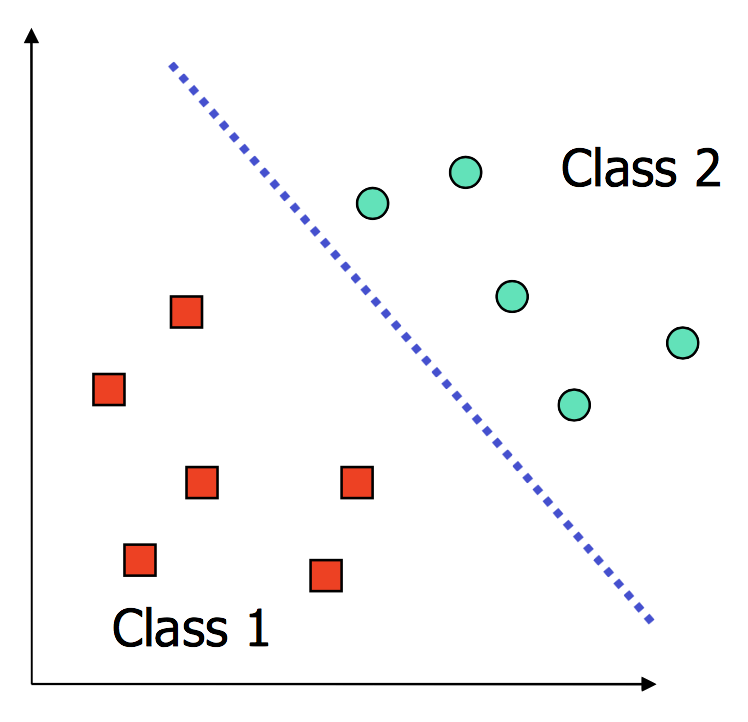
\includegraphics[height=30mm]{lecture18_g1}\quad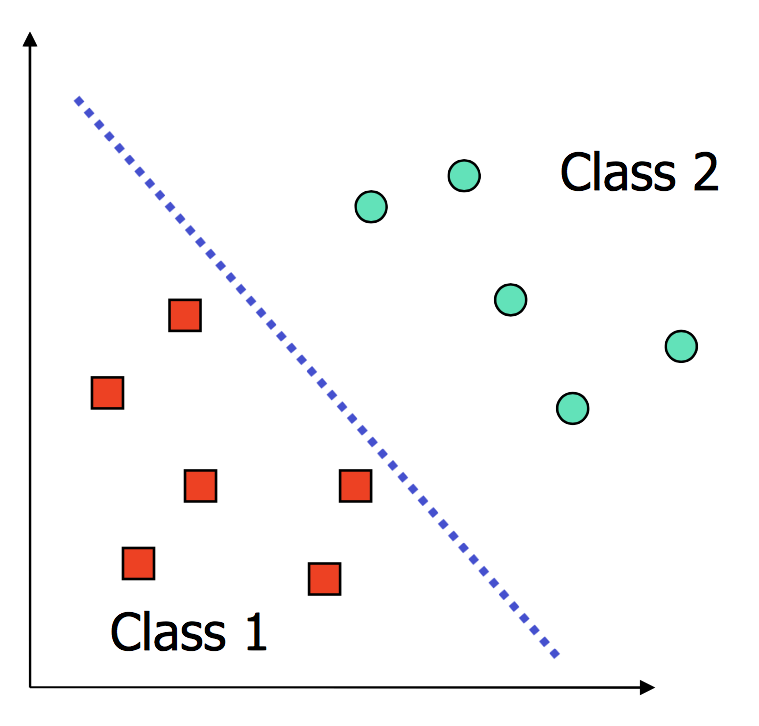
\includegraphics[height=30mm]{lecture18_g2}\quad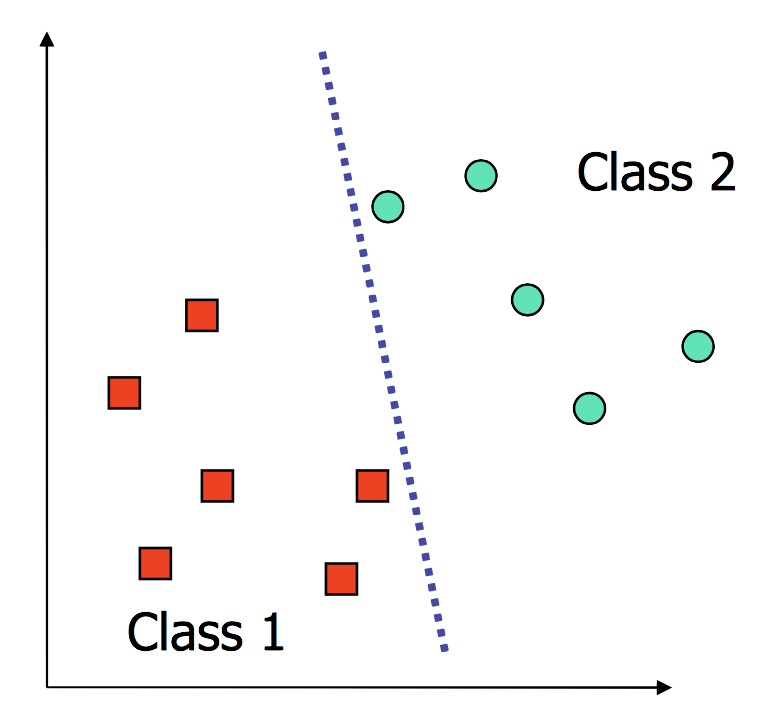
\includegraphics[height=30mm]{lecture18_g3}
\end{center}
\textbf{Question:} What happens to our logistic regression model when training on linearly separable datasets?
}

\only<2-3>{
Constraints on the decision boundary:
\vskip0.2cm
\begin{itemize}
\only<2>{
\item In logistic regression, we typically learn an $\ell_1$ or $\ell_2$ regularized model. 
\vskip0.2cm
So, when the data is linearly separable, we choose a model with the `smallest coefficients'.
\vskip0.2cm
The purpose of regularization is to prevent overfitting.
\vskip0.2cm}
\only<3>{
\item We can consider alternative constraints that prevent overfitting.
\vskip0.2cm
For example, we may prefer a decision boundary that does not `favor' any class (esp. when the classes are roughly equally populous). 
\vskip0.2cm
Geometrically, this means choosing a boundary that maximizes the distance or \emph{margin} between the boundary and both classes.
}
\end{itemize}
}

\only<4>{
\begin{center}
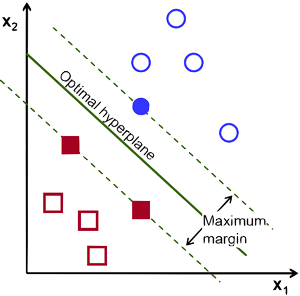
\includegraphics[height=70mm]{lecture18_g4}
\end{center}
}
\end{frame}

%%%%%%%%%%%%%%
\begin{frame}{Geometry to Decision Boundaries} 
\only<1>{
Recall that the decision boundary is defined by some equation in terms of the predictors. A linear boundary is defined by
\[
w^\top x + b = 0 \quad \text{(General equation of a hyperplane)}
\]
Recall that the non-constant coefficients, $w$, represent a \emph{normal vector}, pointing orthogonally away from the plane
\begin{center}
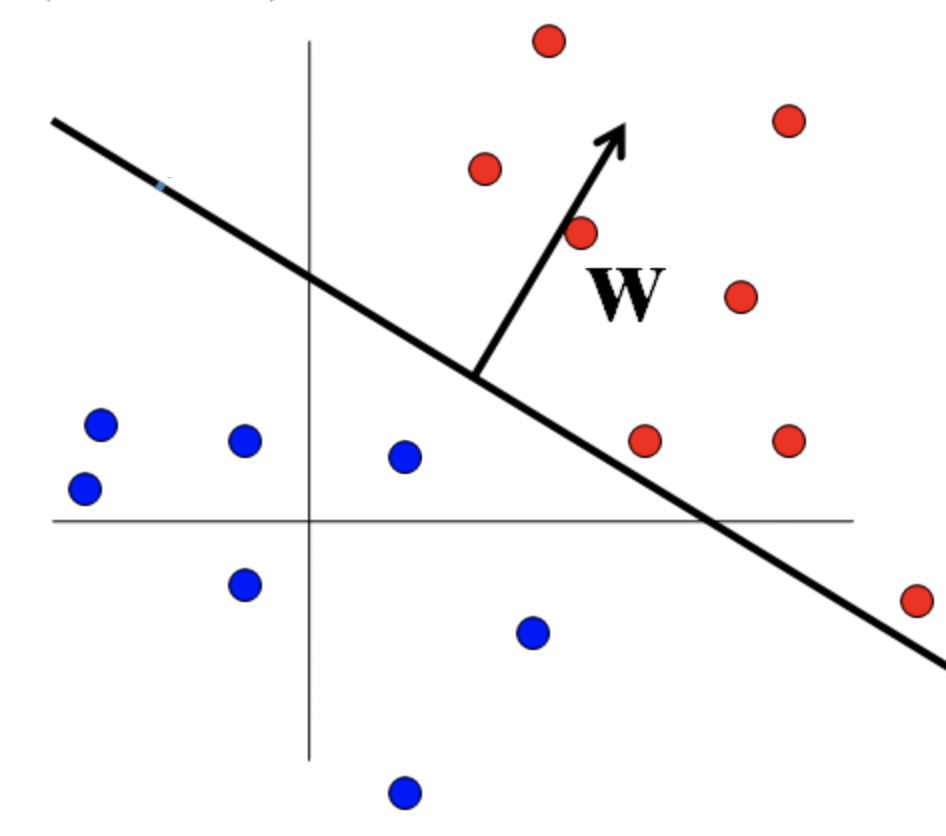
\includegraphics[height=30mm]{lecture18_g5}
\end{center}
}

\only<2>{
\vskip-0.4cm
Now, using some geometry, we can compute the distance between any point to the decision boundary using $w$ and $b$.
\begin{center}
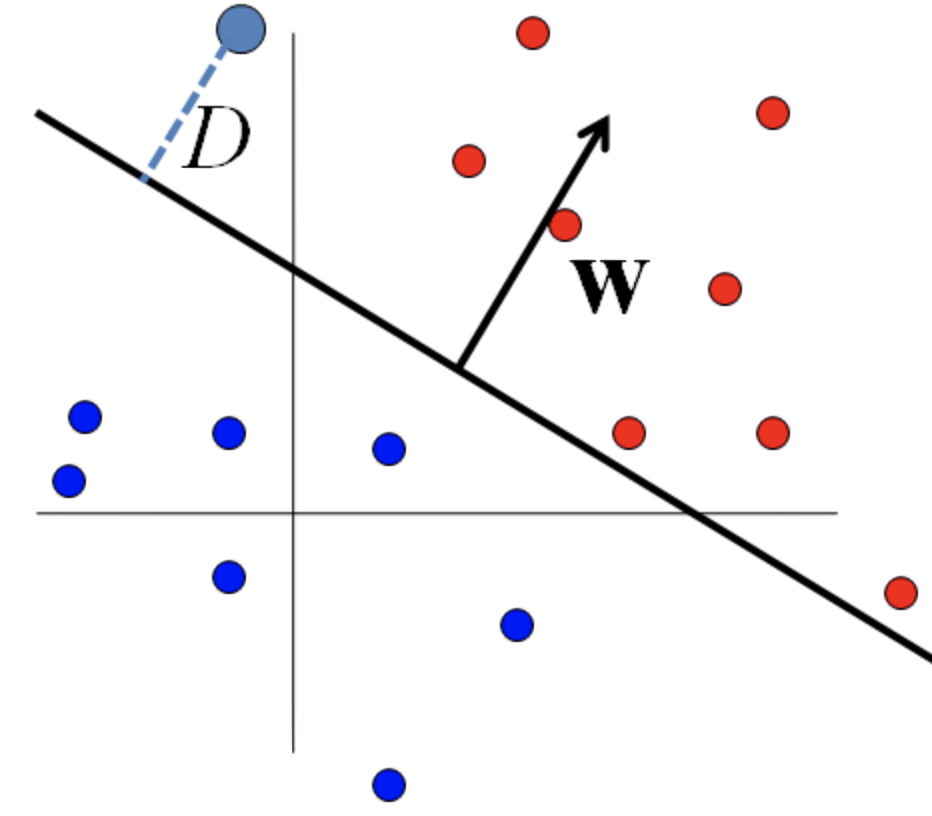
\includegraphics[height=30mm]{lecture18_g6}
\end{center}
The signed distance from a point $x\in \mathbb{R}^n$ to the decision boundary is
\[
D(x) = \frac{w^\top x + b}{\| w\|}\quad \text{(Euclidean Distance Formula)}
\]
}
\end{frame}

%%%%%%%%%%%%%%
\begin{frame}{Maximizing Margins} 
\only<1>{
\vskip-0.4cm
Now we can formulate our goal - find a decision boundary that maximizes the distance to both classes - as an optimization problem
\begin{align*}
\begin{cases}
\max_{w, b} M\\
\text{such that } |D(x_n)| = \frac{y_i(w^\top x_n + b)}{\| w\|} \geq M,\; n = 1, \ldots, N
\end{cases}
\end{align*} 
where $M$ is a real number representing the width of the `margin'. The inequalities $|D(x_n)|\geq M$ are called \emph{constraints}.
\vskip0.2cm
The constrained optimization problem as present here looks tricky. Let's simplify it with a little geometric intuition. 
}

\only<2>{
\vskip-0.4cm
Notice that maximizing the distance of \emph{all points} to the decision boundary, is the exactly the same as maximizing the distance to the \emph{closest points}. 
\vskip0.2cm
The points closest to the decision boundary are called \emph{support vectors}. 
\vskip0.2cm

For any plane, we can always scale the equation 
\[ 
w^\top x + b = 0
\]
so that the support vectors lie on the planes 
\[
w^\top x + b = \pm 1,
\]
depending on their classes.
}

\only<3>{
\vskip-0.4cm
For points on planes $w^\top x + b = \pm 1$, their distance to the decision boundary is $\pm\frac{1}{\|w\|}$. 
\vskip0.2cm
So we can define the \emph{margin} of a decision boundary as the distance to its support vectors, $m = \frac{2}{\|w\|}$
\begin{center}
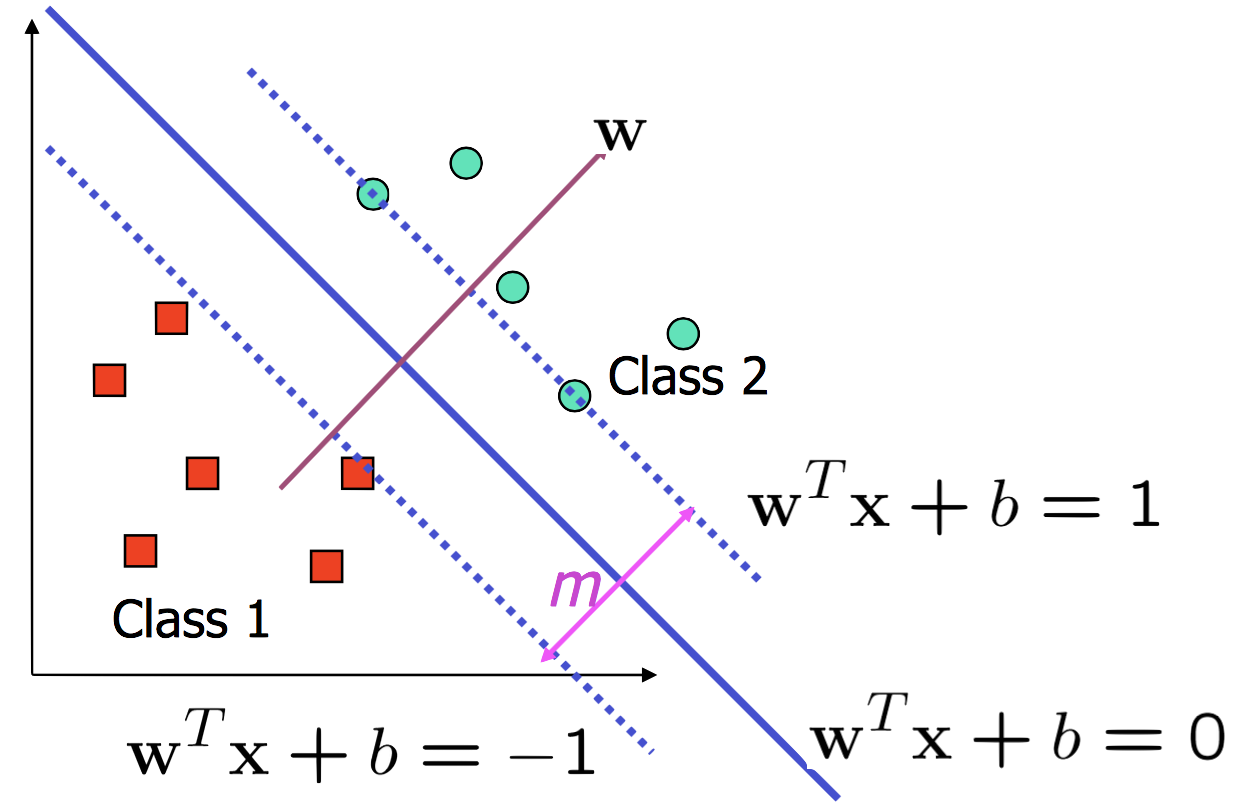
\includegraphics[height=50mm]{lecture18_g7}
\end{center}
}
\end{frame}

%%%%%%%%%%%%%%
\begin{frame}{Support Vector Classifier: Hard Margin} 

Finally, we can reformulate our optimization problem - find a decision boundary that maximizes the distance to both classes - as the maximization of the margin, $m$, \emph{while maintaining zero misclassifications}, 
\[
\begin{cases}
\displaystyle\max_{w, b} \frac{2}{\|w\|}\\
\text{such that } y_n(w^\top x_n + b) \geq 1, \; n = 1, \ldots, N
\end{cases}
\]
The classifier learned by solving this problem is called \emph{hard margin support vector classification}. 
\vskip0.2cm
Often SVC is presented as a minimization problem:
\[
\begin{cases}
\displaystyle\min_{w, b} {\|w\|^2}\\
\text{such that } y_n(w^\top x_n + b) \geq 1, \; n = 1, \ldots, N
\end{cases}
\]
\end{frame}

%%%%%%%%%%%%%%
\begin{frame}{SVC and Convex Optimization} 
\vskip-0.4cm
As a convex optimization problem SVC has been extensively studied and can be solved by a variety of algorithms
\vskip0.2cm
\begin{itemize}
\item \textbf{(Stochastic)} libLinear 
\vskip0.2cm
Fast convergence, moderate computational cost
\item \textbf{(Greedy)} libSVM
\vskip0.2cm
Fast convergence, moderate computational cost
\item \textbf{(Stochastic)} Stochastic Gradient Descent
\vskip0.2cm
Slow convergence, low computational cost per iteration
\item \textbf{(Greedy)} Quasi-Newton Method 
\vskip0.2cm
Very fast convergence, high computational cost
\end{itemize}
\end{frame}


%%%%%%%%%%%%%%%%%%%%%%%%%%%%%%%%%%%%%%%%%%%%%%%%%%%%%%%%%%%%%%%%%%%%%%%%%%%%%%
\section{Classifying Linear Non-Separable Data}

%%%%%%%%%%%%%%
\begin{frame}{The Margin/Error Trade-Off} 
\vskip-0.4cm
Maximizing the margin is a good idea as long as we assume that the underlying classes are linear separable and that the data is noise free. 
\vskip0.2cm
If data is noisy, we might be sacrificing generalizability in order to minimize classification error with a very narrow margin 
\begin{center}
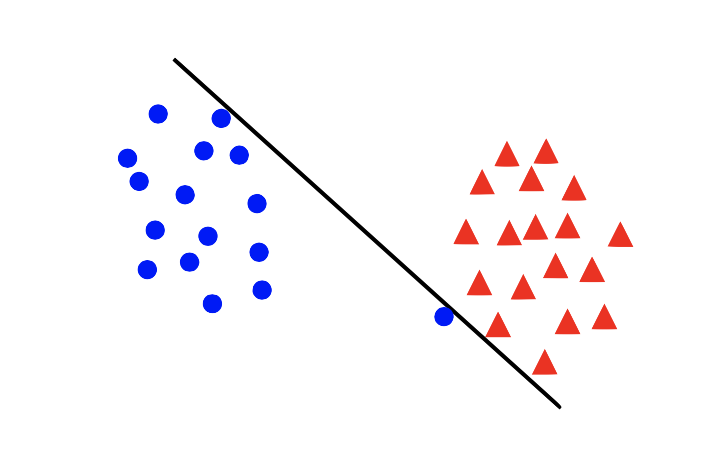
\includegraphics[height=30mm]{lecture18_g8}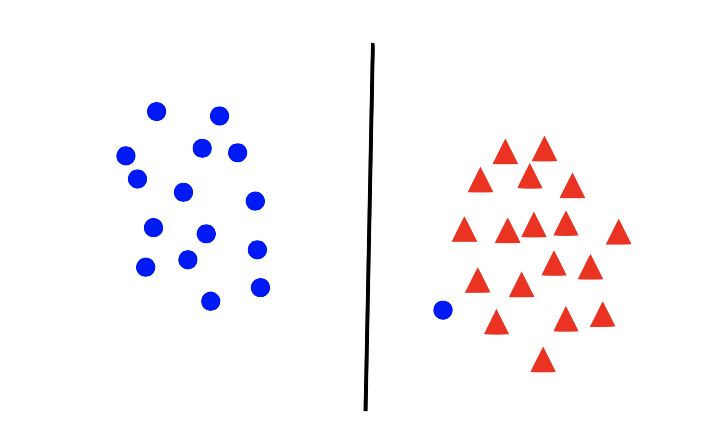
\includegraphics[height=30mm]{lecture18_g9}
\end{center}
With every decision boundary, there is a trade-off between maximizing margin and minimizing the error.
\end{frame}

%%%%%%%%%%%%%%
\begin{frame}{Support Vector Classifier: Soft Margin}
\only<1>{
Since we want to balance maximizing the margin and minimizing the error, we want to use an objective function that takes both into account:
\[
\begin{cases}
\displaystyle \min_{w, b} {\|w\|^2} + \alert{\lambda\text{Error}(w, b)}\\
\text{such that } y_n(w^\top x_n + b) \geq 1, \; n = 1, \ldots, N
\end{cases}
\]
where $\lambda$ is an intensity parameter. 
\vskip0.2cm
So just how should we compute the error for a given decision boundary? 
}

\only<2>{
\vskip-0.4cm
We want to express the error as a function of distance to the decision boundary. 
\vskip0.2cm
Recall that the support vectors have distance $1/\|w\|$ to the decision boundary. We want to penalize two types of `errors'
\vskip0.2cm
\begin{itemize}
\item \textbf{(margin violation)} points that are on the correct side of the boundary but is inside the margin. They have distance $\xi/\|w\|$, where $0< \xi <1$. 
\vskip0.2cm
\item \textbf{(misclassification)} points that are on the wrong side of the boundary. They have distance $\xi/\|w\|$, where $\xi>1$. 
\end{itemize}
\vskip0.2cm
Specifying a nonnegative quantity for $\xi_n$ is equivalent to quantifying the error on the point $x_n$. 
}

\only<3>{
\begin{center}
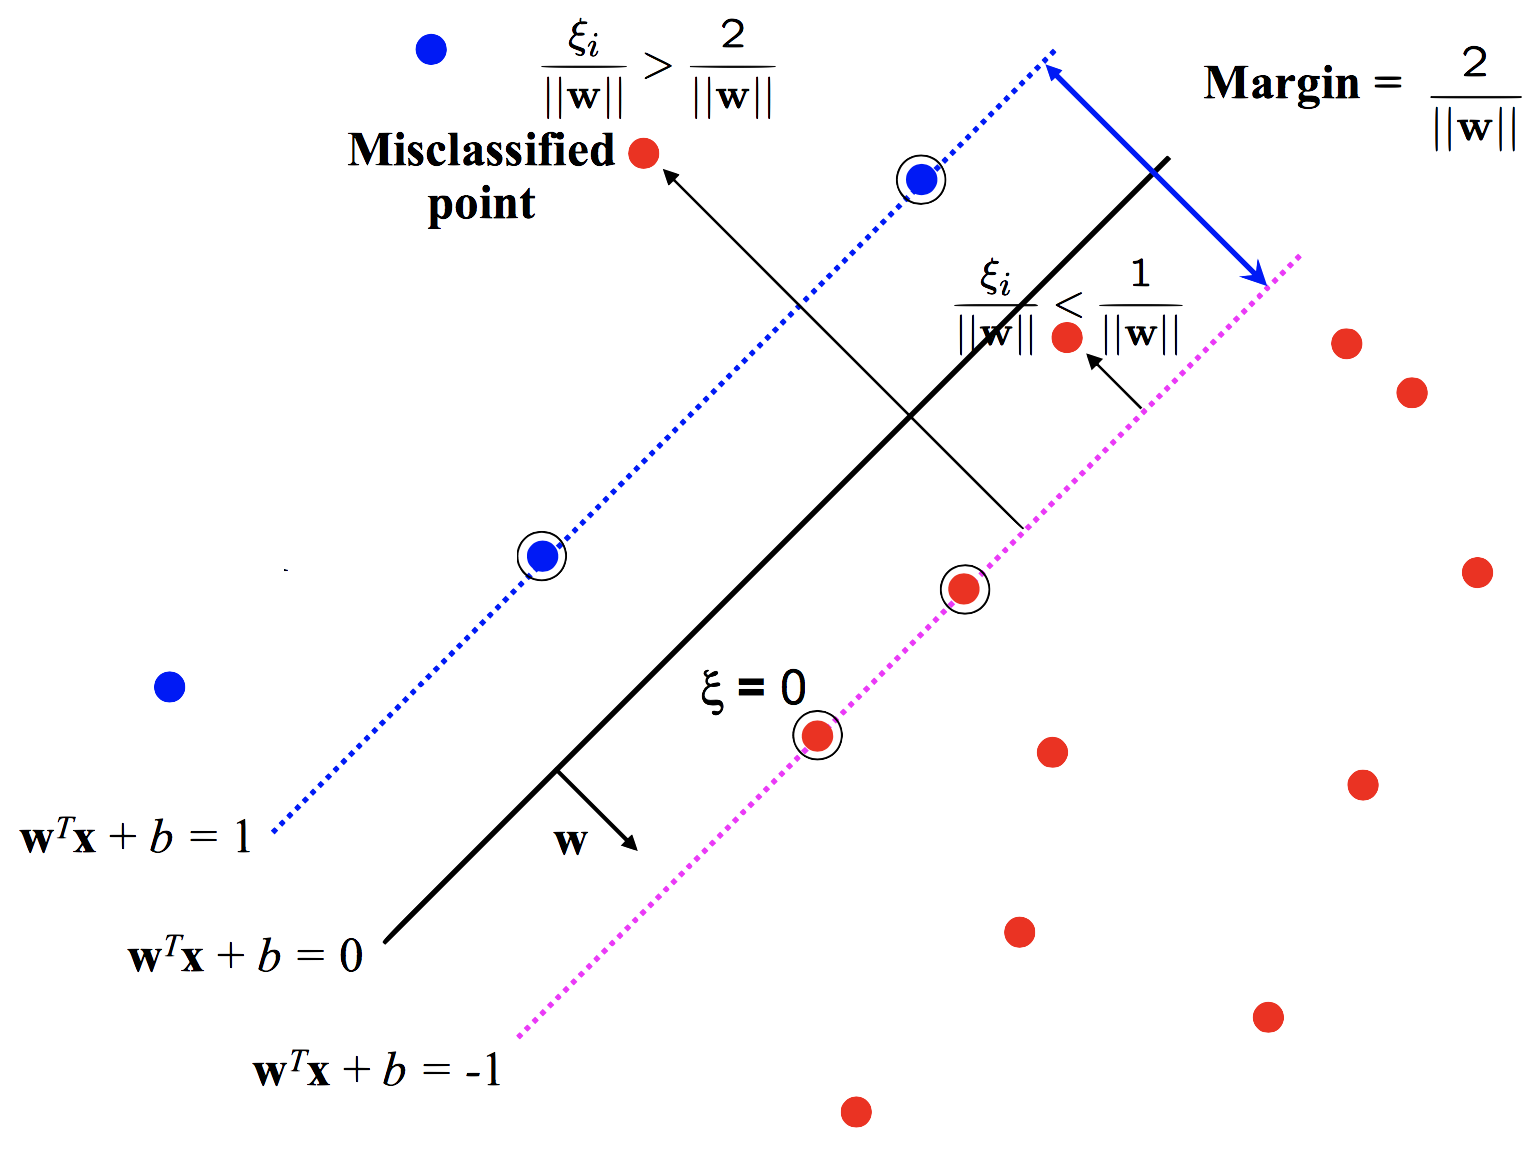
\includegraphics[height=70mm]{lecture18_g10}
\end{center}
}

\only<4>{
Formally, we incorporate error terms $\xi_n$'s into our optimization problem by:
\[
\begin{cases}
\displaystyle \min_{\xi_n \in \mathbb{R}^{+}, w, b} \|w\|^2 + \alert{\lambda\sum_{n=1}^N \xi_n}\\
\text{such that } y_n(w^\top x_n + b) \geq 1 - \alert{\xi_n}, \; n = 1, \ldots, N
\end{cases}
\]
The solution to this problem is called \emph{soft margin support vector classification} or simply \emph{support vector classification}.
}
\end{frame}

%%%%%%%%%%%%%%
\begin{frame}{Tuning SVC} 
\vskip-0.4cm
\small
Choosing different values for $\lambda$ in 
\[
\begin{cases}
\displaystyle \min_{\xi_n \in \mathbb{R}^{+}, w, b} \|w\|^2 + \alert{\lambda\sum_{n=1}^N \xi_n}\\
\text{such that } y_n(w^\top x_n + b) \geq 1 - \alert{\xi_n}, \; n = 1, \ldots, N
\end{cases}
\]
will give us different classifiers.
\vskip0.2cm
In general, 
\begin{itemize}
\item small $\lambda$ penalizes errors less and hence the classifier will have a large margin
\item large $\lambda$ penalizes errors more and hence the classifier will accept narrow margins to improve classification
\item setting $\lambda = \infty$ produces the hard margin solution
\end{itemize}
\end{frame}

%%%%%%%%%%%%%%
\begin{frame}{Example} 
[Compare different classifiers]

[Investigate variance]
\end{frame}

\end{document}
